%!TEX root = thesis.tex

\chapter{Visualisation Design}
\label{chap:visualisation-design}

Following the exploratory field study (see Chapter~\ref{chap:exploratory-field-study}), a strategy for visualisation prototyping and evaluation was developed. The field study indicated a need for further investigation of the application of visualisations to the live coding process. This chapter outlines the reasoning behind developing a set of prototype visualisations, the process of development and the resulting software prototype.

% {\color{red}\cite{Ware2013a,McLean2010a,Purchase1996} will be useful here.}

\section{Rationale}

{\color{red} how did the exploratory field study contribute? }

Evaluation of the literature identified the need for visualisations that helped live coding audiences understand and enjoy the live coding performance. To this end, two sets of visualisations were developed. The first was intended to increase the enjoyment of the audience, enhancing aesthetic appeal and was labelled the ``aesthetic condition''. The second was intended to communicate the live coding process, help the audience to understand the programmatic aspects of the performance and was labelled the ``didactic condition''.

\section{Requirements}

In order to systematically and efficiently develop a visualisation design strategy, two stakeholders were identified. These included the live coder and the intended audience.

Evaluation of the visualisation prototype required application to a live coding performance. To achieve this, the live coder would need to apply the visualisations to a live performance. To this end, discussions with the live coder identified functional requirements including simultaneous display of source code and visualisations and visualisations depicting the progression of the performance accurately. Non-functional requirements identified included performance, as the nature of live coding is realtime, and reliability, as a single failure in the visualisations could cause catastrophic failure within the live coding performance.

The intended audience was identified as a critical stakeholder in the ultimate effectiveness of the visualisations developed. The audience evaluated in the initial field study would provide the basis for these requirements. 

% -discuss audience requirements identified from first study

\section{Risks}

In the early stages of the development of a visualisation strategy, a number of risks were identified. Discussion of the risk management strategy are outlined below.

Fundamental to live coding is the performance element. Live coding requires a reliable programming environment. Visualisations developed for this environment required that the chance of failure were minimised. To mitigate the chance of a failure in the live coding environment, a test strategy was developed for the visualisations to ensure that they did not cause unrecoverable failures and did not cause memory leaks.

Timeline constraints were also identified as a potential risk factor in the development and evaluation of the visualisations. Mitigation involved developing a flexible, iteration based development plan with estimated milestones.
% {\color{red} Add timeline in here......}

-risk that the visualisations would not provide any benefit or would negatively impact the performance... mitigated by the iteration based approach to developing the visualisations

-risk that the visualisations would interfere with the live coder...

% -risk that the visualisations were not the correct strategy to begin with?

\section{Design}

\begin{figure}
  \centering 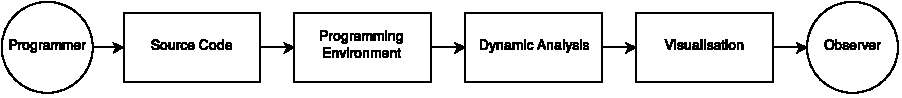
\includegraphics[width=\columnwidth]{../images/diagrams/knowledge-flow-initial.pdf}
  \caption{Knowledge flow from programmer to observer as directed by the visualisation technique employed.}
\label{fig:knowledge-flow-initial}
\end{figure}


The intial iteration of the visualisation prototype consisted of two separate conditions. {\color{red} Where did the idea for these two conditions come from?} Each condition consisted of four visual progressions with the intention of representing the addition and removal of instruments during the live coding performance.

The first visualisation condition was labelled the ``aesthetic'' condition reflecting the intention to improve enjoyment during the live coding performance. The second visualisation condition was labelled the ``didactic'' condition with an intended goal of improving understanding during the live coding performance.

% The design of the initial visualisations focussed on the application of the literature on visualisation design to the field of software visualisation and the application to the visualisation of live code.

-guidelines set out by mclean were used in understanding the application of visualisation to live coding...
\cite{McLean2010a}...

-guidelines set out by ware were used in developing the visualisations...
% - what are the guidelines used
\cite{Ware2013a}...

Cairo was used as the supporting graphics library for visualisations implementation with the final prototype consisting of 1000 \ac{SLOC}. Visualisations were written in pure xtlang, as part of the Extempore live coding environment.

\afterpage{
\begin{figure}
\centering
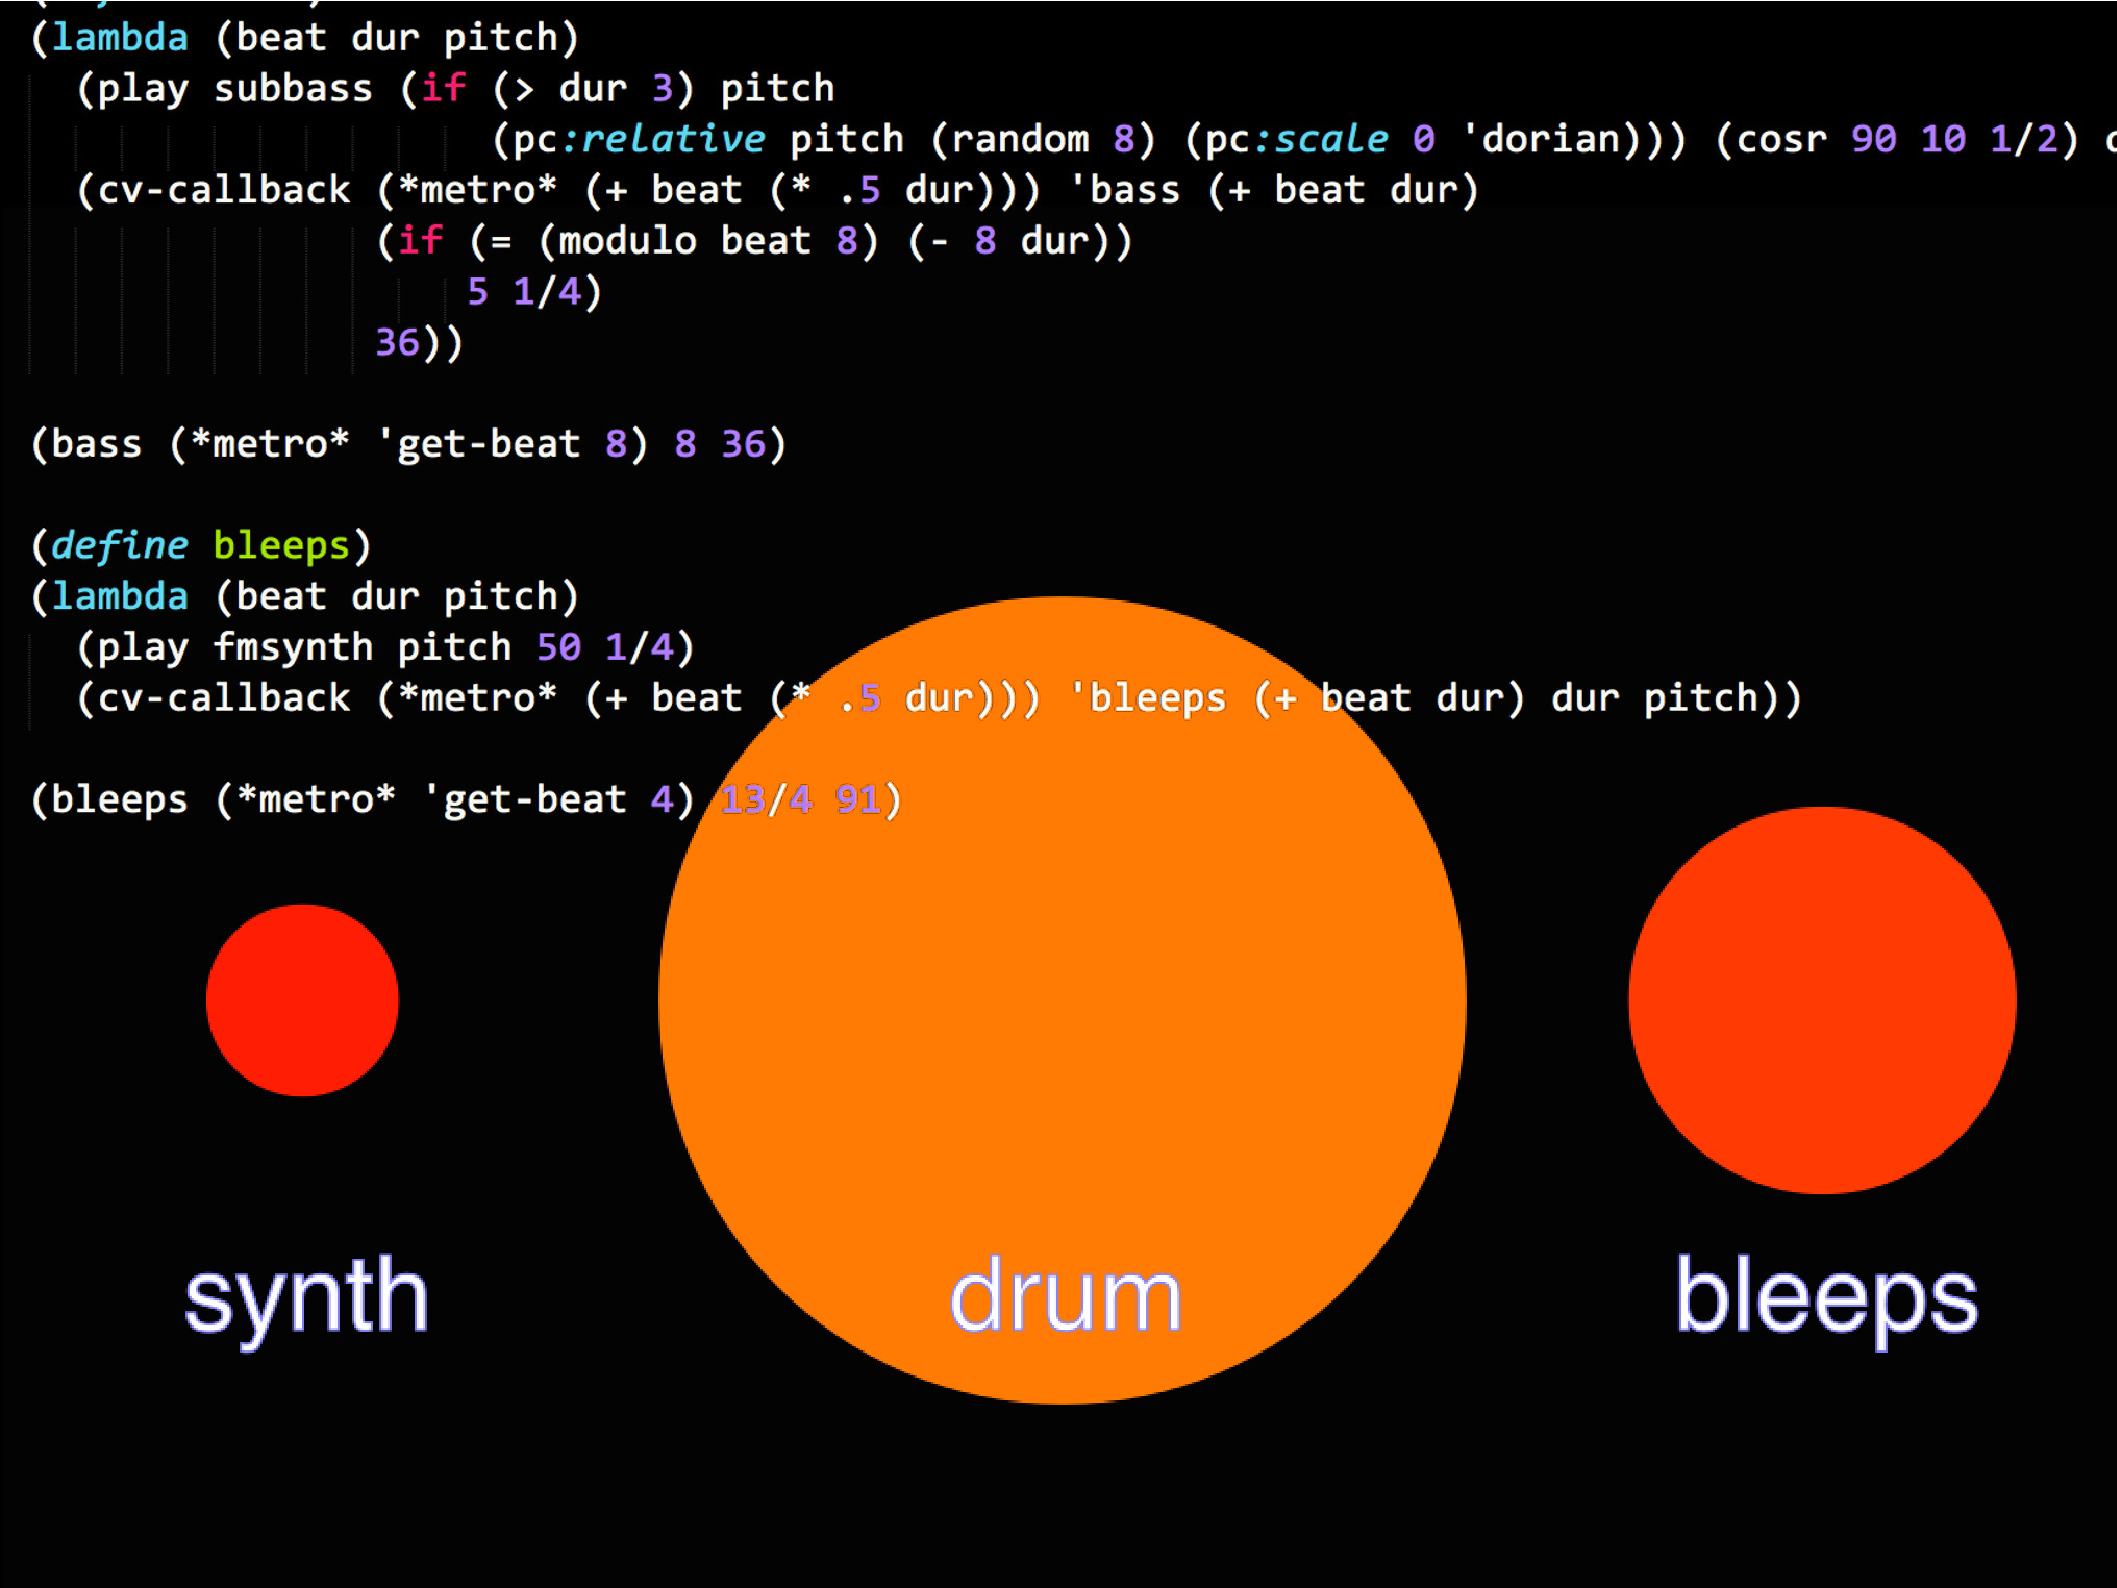
\includegraphics[width=0.75\columnwidth]{../study-2/results/visualisations/didactic-vis-overlay}
\caption{An example didactic visualisation.}
\label{fig:didactic-visualisation}
\end{figure}

\begin{figure}
\centering
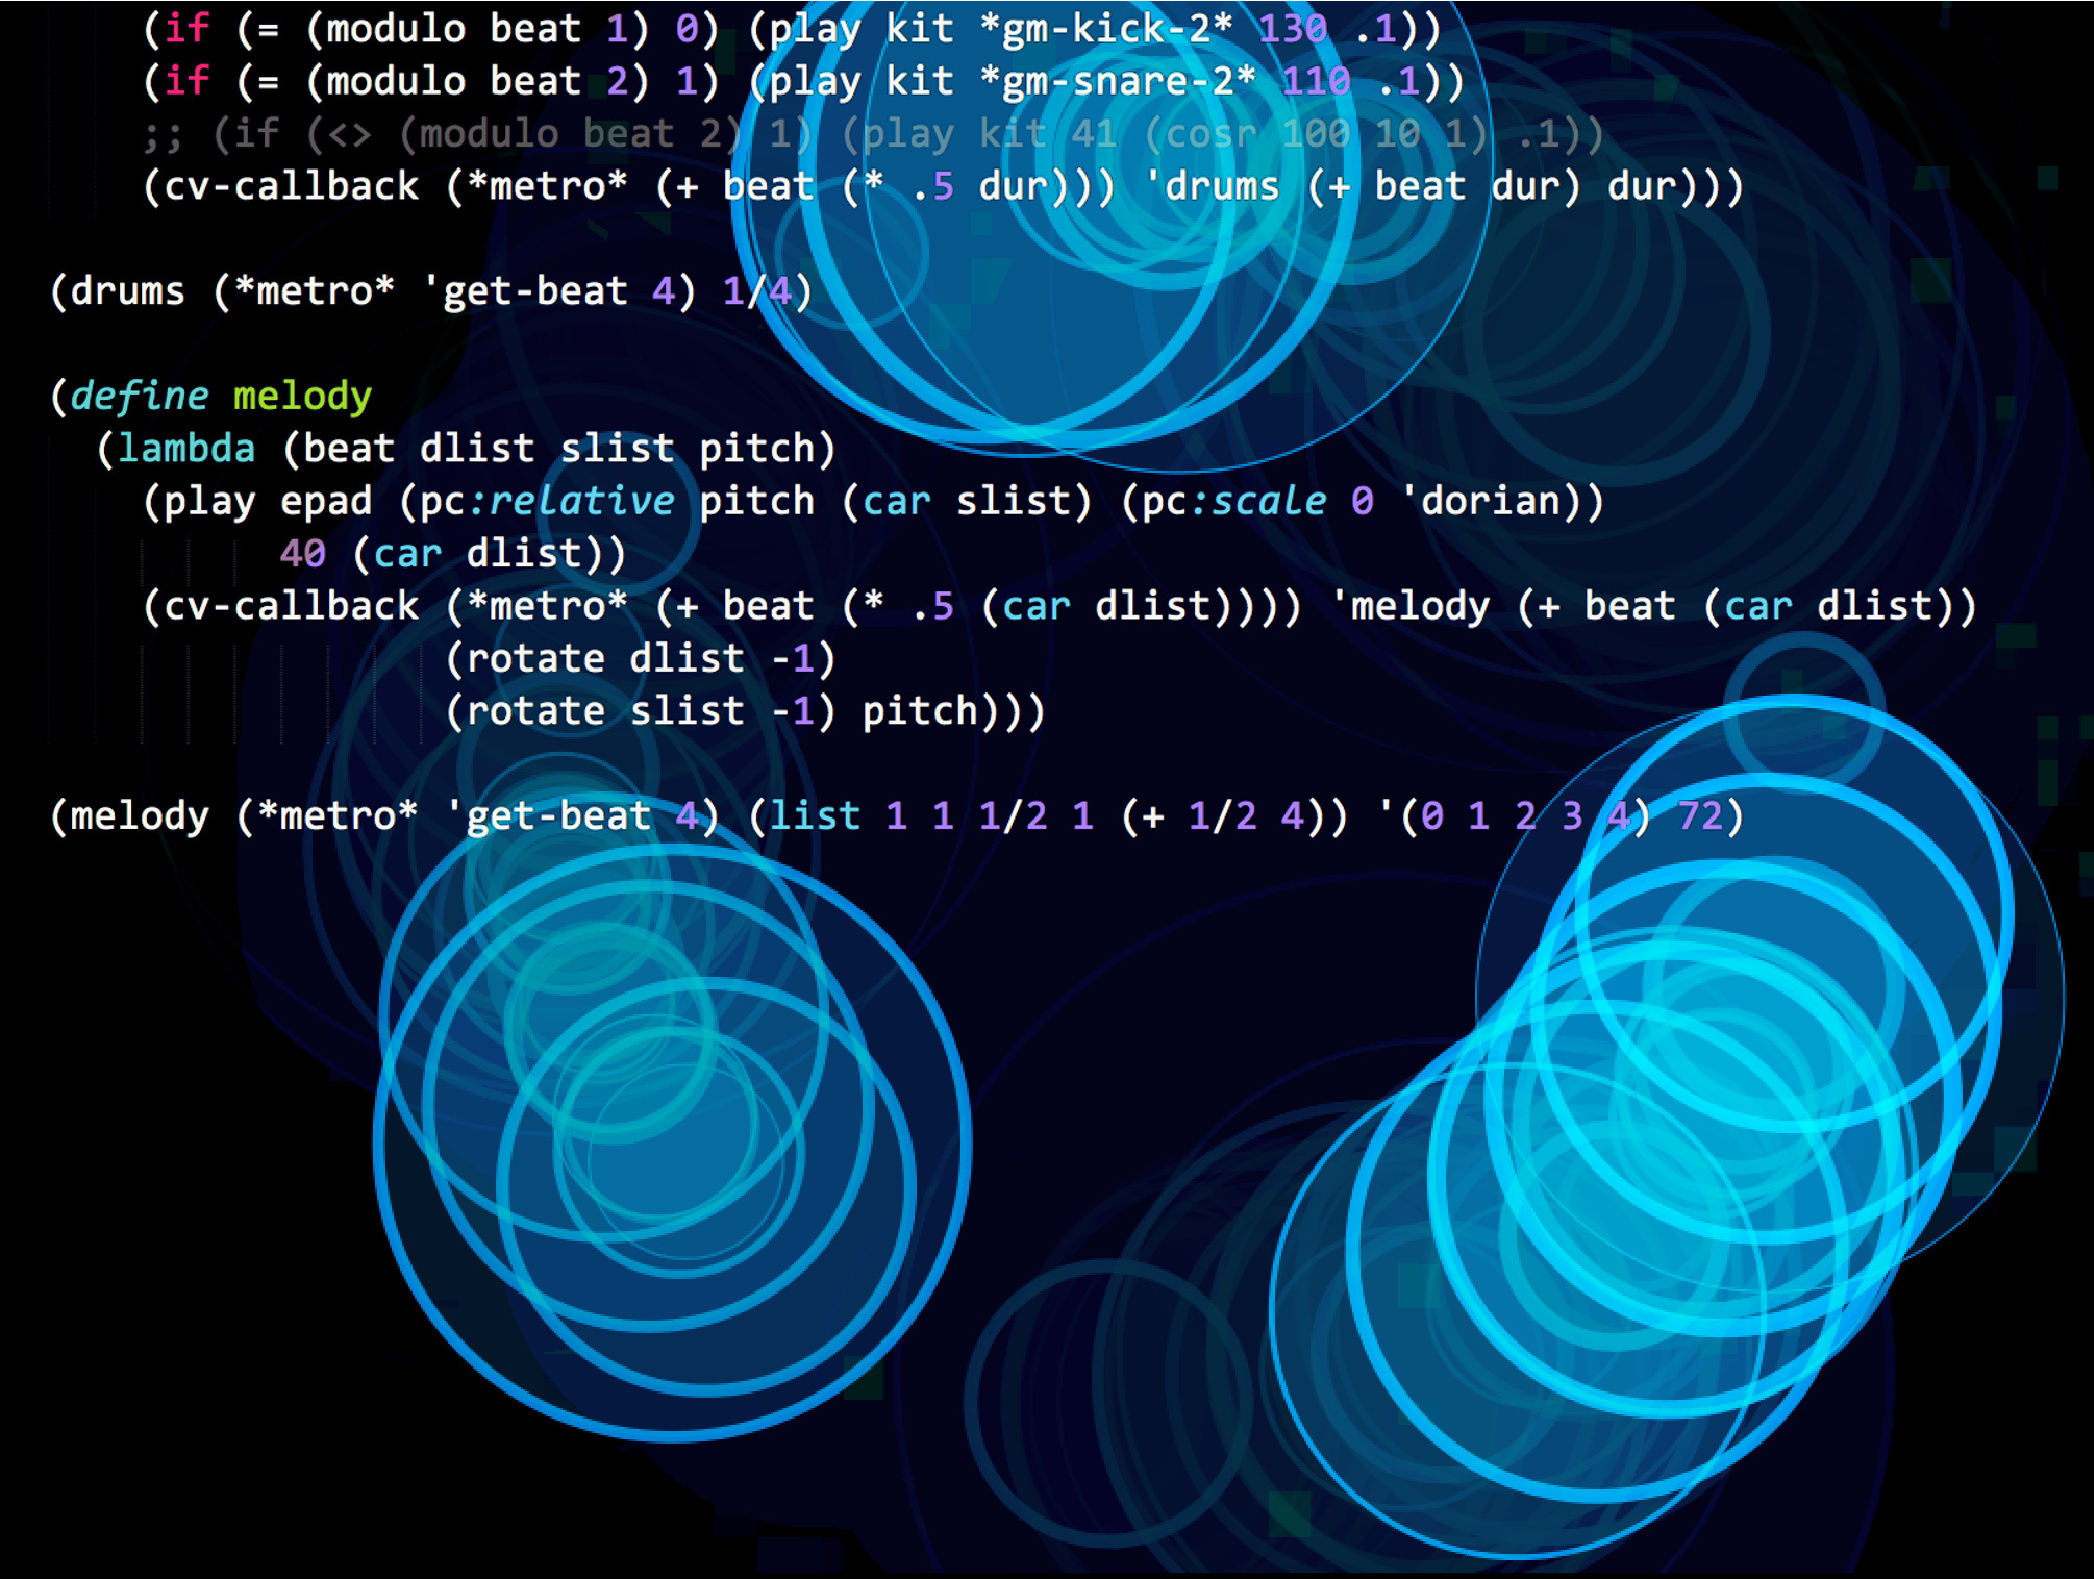
\includegraphics[width=0.75\columnwidth]{../study-2/results/visualisations/aesthetic-vis-overlay}
\caption{An example aesthetic visualisation.}
\label{fig:aesthetic-visualisation}
\end{figure}
\clearpage}

Visualisations developed employed dynamic analysis of the running code to generate the visuals. The intended knowledge flow from programmer to observer is shown in Figure~\ref{fig:knowledge-flow-initial}.

Music visualisation is an extremely rich and open-ended task, so to guide the development of the visualisations for our lab study, we used the concepts of understanding and enjoyment from the initial survey to develop two new code visualisations: a \emph{didactic} one and an \emph{aesthetic} one. 

\subsection{Didactic Visualisation}
\label{sec:didactic-visualisation}

The didactic visualisation (shown in Figure~\ref{fig:didactic-visualisation}) attempted to communicate \emph{information} about the actions of the programmer, prominently displaying the \emph{names} of the active (source code) functions and the ``time until next execution'' for each function (which is particularly relevant in a time-sensitive programming context such as music making). Bright colours and solid shapes were used to ensure constant visibility and to communicate the intention of the underlying code. The didactic visualisations proceeded through four stages, with progression made depending on the number of active functions (instruments).

\subsection{Aesthetic Visualisation}
\label{sec:aesthetic-visualisation}

The aesthetic visualisation technique was designed to react to the programmer's activity in a more abstract way, to maximise aesthetic appeal~\cite{Cawthon2007} and to engage the audience's interest. Although still based on the source code and the livecoder's edits, the generation of shapes was driven by instrument volume and synchronised with the musical beat. The emphasis for the aesthetic visualisation was on the artistic appeal of the visuals (see Figure~\ref{fig:aesthetic-visualisation}), including more variety in visual structure and colour. As in the didactic condition, the aesthetic visualisations proceeded through four stages, based on the number of active functions (instruments), but these visuals had no textual labels and they moved and interacted with each other over the entire projected scene.

\section{Summary}

Evaluation of the visualisation technique was required 
-needed to test out the assumptions made while designing the visualisation prototype
-wanted to compare the two visualisation techniques
-compare the two techniques and build on this for future iterations



